\subsubsection{Package com.sirius.sequenziatore.server.presenter.user}
\begin{figure}[H] \centering 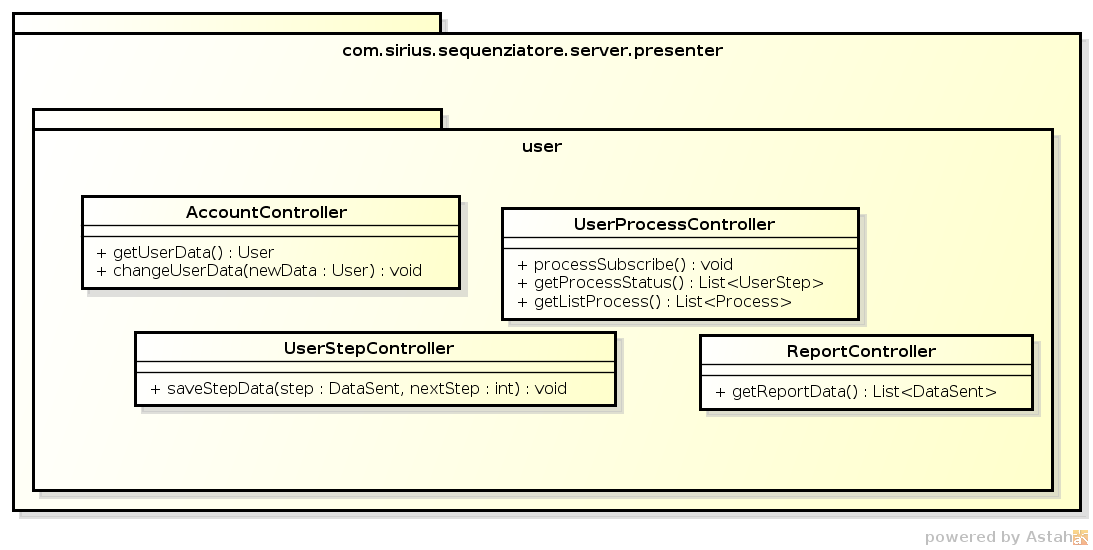
\includegraphics[width=%
\textwidth]
{./classi/server/presenteruser.png} \caption{Diagramma package - \texttt{com.sirius.sequenziatore.server.presenter.user}}
\end{figure}
\paragraph{UserStepController}%----------------------------------------------------------------%
\
\begin{figure}[H] \centering
\includegraphics[trim=0cm 0.8cm 0cm 0cm,clip=true,scale=0.75]%
{./classi/server/userstepcontroller.png} \caption{Diagramma classe - \texttt{UserStepController}}
\end{figure}
\begin{itemize}
	\item \textbf{Descrizione: } Questa classe gestisce la ricezione dei dati di un passo inviati da un utente tramite una richiesta di tipo \textit{POST}, tale passo dovrà essere inserito nel database, ponendo attenzione se è un passo che richiede approvazione o meno;
	\item \textbf{Mappatura base: } \textit{\textbackslash stepdata\textbackslash user}
	\item \textbf{Relazioni con altri componenti: }
	La classe utilizzerà le seguenti classi:
	\begin{itemize}
		\item \texttt{com.sirius.sequenziatore.server.model.DataSent;}
		\item \texttt{com.sirius.sequenziatore.server.model.UserStep;}
		\item \texttt{com.sirius.sequenziatore.server.model.StepDao;}
	\end{itemize}
	tramite le interfacce:
	\begin{itemize}
		\item \texttt{com.sirius.sequenziatore.server.model.ITransferObject;}
		\item \texttt{\sModel .IDataAccessObject;}
	\end{itemize}
	\item \textbf{Metodi: }\begin{itemize}
					\item \texttt{+void saveStepData(DataSent step,int nextStep):}\\
					questo metodo gestisce una richiesta \textbf{POST} da un utente, riceve i dati inerenti a un passo e li inserisce nel database e se non necessita di approvazione lo segna come completato e modifica quale sarà il passo o i passi che si potranno eseguire; 
				\end{itemize}
\end{itemize}
\paragraph{UserProcessController}%----------------------------------------------------------------%
\
\begin{figure}[H] \centering
\includegraphics[trim=0cm 0.8cm 0cm 0cm,clip=true,scale=0.75]%
{./classi/server/userprocesscontroller.png} \caption{Diagramma classe - \texttt{UserProcessController}}
\end{figure}
\begin{itemize}
	\item \textbf{Descrizione: } Questa classe permette all' utente varie operazioni, innanzitutto l' iscrizione ad un processo, poi restituisce il passo a cui è arrivato e il suo stato per tale processo e infine fornisce una lista di processi con tutti i processi a cui si può iscrivere e i processi per i quali può chiedere di fare il \textit{report};
	\item \textbf{Mappatura base: } \textit{\textbackslash user\textbackslash \{username\}}
	\item \textbf{Relazioni con altri componenti: }
	La classe utilizzerà le seguenti classi:
	\begin{itemize}
		\item \texttt{com.sirius.sequenziatore.server.model.Process;}
		\item \texttt{com.sirius.sequenziatore.server.model.UserStep;}
		\item \texttt{com.sirius.sequenziatore.server.model.ProcessDao;}
		\item \texttt{com.sirius.sequenziatore.server.model.StepDao;}
	\end{itemize}
	tramite le interfacce:
	\begin{itemize}
		\item \texttt{com.sirius.sequenziatore.server.model.ITransferObject;}
		\item \texttt{\sModel .IDataAccessObject;}
	\end{itemize}
	\item \textbf{Metodi: }\begin{itemize}
					\item \texttt{+void processSubscribe()}:\\
					questo metodo mappa su \textit{\textbackslash subscribe\textbackslash \{processid\}} e gestisce una richiesta di tipo \textbf{POST} che permette ad un utente di iscriversi al processo voluto;
					\item \texttt{+List<UserStep> getProcessStatus()}:\\
					questo metodo mappa su \textit{\textbackslash subscribe\textbackslash \{processid\}} e gestisce una richiesta \textbf{GET} che restituisce all' utente il proprio status per tale processo, restituendo il passo o i passi che può eseguire e quanti passi ha completato del processo;
					\item \texttt{+List<Process> getListProcess()}:\\
					questo processo mappa su \textit{\textbackslash processlist} e gestisce una richiesta di tipo \textbf{GET} andando e restituire una lista di processi che contiene tutti i processi  a cui è iscritto e quelli a cui si può iscrivere;
				\end{itemize}
\end{itemize}
\paragraph{AccountController}%----------------------------------------------------------------%
\
\begin{figure}[H] \centering
\includegraphics[trim=0cm 0.8cm 0cm 0cm,clip=true,scale=0.75]%
{./classi/server/accountcontroller.png} \caption{Diagramma classe - \texttt{AccountController}}
\end{figure}
\begin{itemize}
	\item \textbf{Descrizione: } Classe che fornisce i dati di un utente e ne permette la modifica dei suddetti;
	\item \textbf{Mappatura base: } \textit{\textbackslash account\textbackslash \{username\}}
	\item \textbf{Relazioni con altri componenti: }
	La classe utilizzerà le seguenti classi:
	\begin{itemize}
		\item \texttt{com.sirius.sequenziatore.server.model.User;}
		\item \texttt{com.sirius.sequenziatore.server.model.UserDao;}
	\end{itemize}
	tramite le interfacce:
	\begin{itemize}
		\item \texttt{com.sirius.sequenziatore.server.model.ITransferObject;}
		\item \texttt{\sModel .IDataAccessObject;}
	\end{itemize}
	\item \textbf{Metodi: }\begin{itemize}
					\item \texttt{+User getUserData():}\\
					questo metodo gestisce una richiesta di tipo \textbf{GET} e restituisce un oggetto di tipo User contenente tutti i dati di un utente;
					\item \texttt{+void changeUserData(User newData):}\\
					questo metodo gestisce una chiamata di tipo \textbf{POST} e permette la modifica dei dati di un account di un utente;
				\end{itemize}
\end{itemize}
\paragraph{ReportController}%----------------------------------------------------------------%
\
\begin{figure}[H] \centering
\includegraphics[trim=0cm 0.8cm 0cm 0cm,clip=true,scale=0.75]%
{./classi/server/reportcontroller.png} \caption{Diagramma classe - \texttt{ReportController}}
\end{figure}
\begin{itemize}
	\item \textbf{Descrizione: } Questa classe fornirà al client tutti i dati necessari per creare il report di un utente per un certo processo;
	\item \textbf{Mappatura base: } \textit{\textbackslash report\textbackslash \{username\}\textbackslash \{processid\}}
	\item \textbf{Relazioni con altri componenti: }
	La classe utilizzerà le seguenti classi:
	\begin{itemize}
		\item \texttt{com.sirius.sequenziatore.server.model.User;}
		\item \texttt{com.sirius.sequenziatore.server.model.Process;}
		\item \texttt{\sModel .Step;}
		\item \texttt{\sModel .UserDao;}
		\item \texttt{\sModel .ProcessDao;}
		\item \texttt{\sModel .StepDao;}
		
	\end{itemize}
	tramite le interfacce:
	\begin{itemize}
		\item \texttt{com.sirius.sequenziatore.server.model.ITransferObject;}
		\item \texttt{\sModel .IDataAccessObject;}
	\end{itemize}
	\item \textbf{Metodi: }\begin{itemize}
					\item \texttt{+List<DataSent> getReportData():}\\
					questo metodo gestisce una richiesta di tipo \textbf{GET} e fornirà tutti i dati inseriti da un utente per un certo processo;
				\end{itemize}
\end{itemize}